\section{Estado Actual Frente al de Referencia}

\subsection{Conociendo el estado actual}

Con la notación de las arquitecturas objetivo establecidas, al igual que el desarrollo del módulo encargado de la construcción y validación de los archivos de configuración; lo siguiente era la definición del proceso de la comparación entre la arquitectura actual y la arquitectura de referencia. Este proceso, nos permitirá evaluar el estado del sistema y, por consiguiente, establecer las acciones a tomar con el fin de adaptar la arquitectura hacia el estado objetivo establecido.

Esto requiere conocer el estado actual del sistema, al igual que el conocer el estado objetivo. Siendo así, y ya teniendo la posibilidad de declarar las necesidades de la aplicación, lo siguiente es establecer una manera de determinar el estado del sistema. Dado el enfoque hacia los datos recolectados, es necesario el precisar la manera en la que conoceríamos en qué estado se encuentra el sistema.

Partiendo de esto, lo primero era el identificar los puntos de acceso por los cuales podríamos acceder a los datos, en el caso de Smart Campus UIS, como se observa en la figura \ref{fig:ArquitecturaSmartCampus}, hay dos maneras en las que podemos acceder a los datos. La primera, es haciendo consultas a la base de datos en la cual se guardan los registros; la segunda, implica recibir los mensajes que viajan por el bus de datos, sea el de los adaptadores de descripción o el de los dispositivos con el servicio de mensajería , y procesar cada uno de los mensajes.

\begin{figure}[ht]
    \centering
    \caption{Arquitectura del prototipo de Smart Campus definido por }\citeA{msc_henry_2022}
    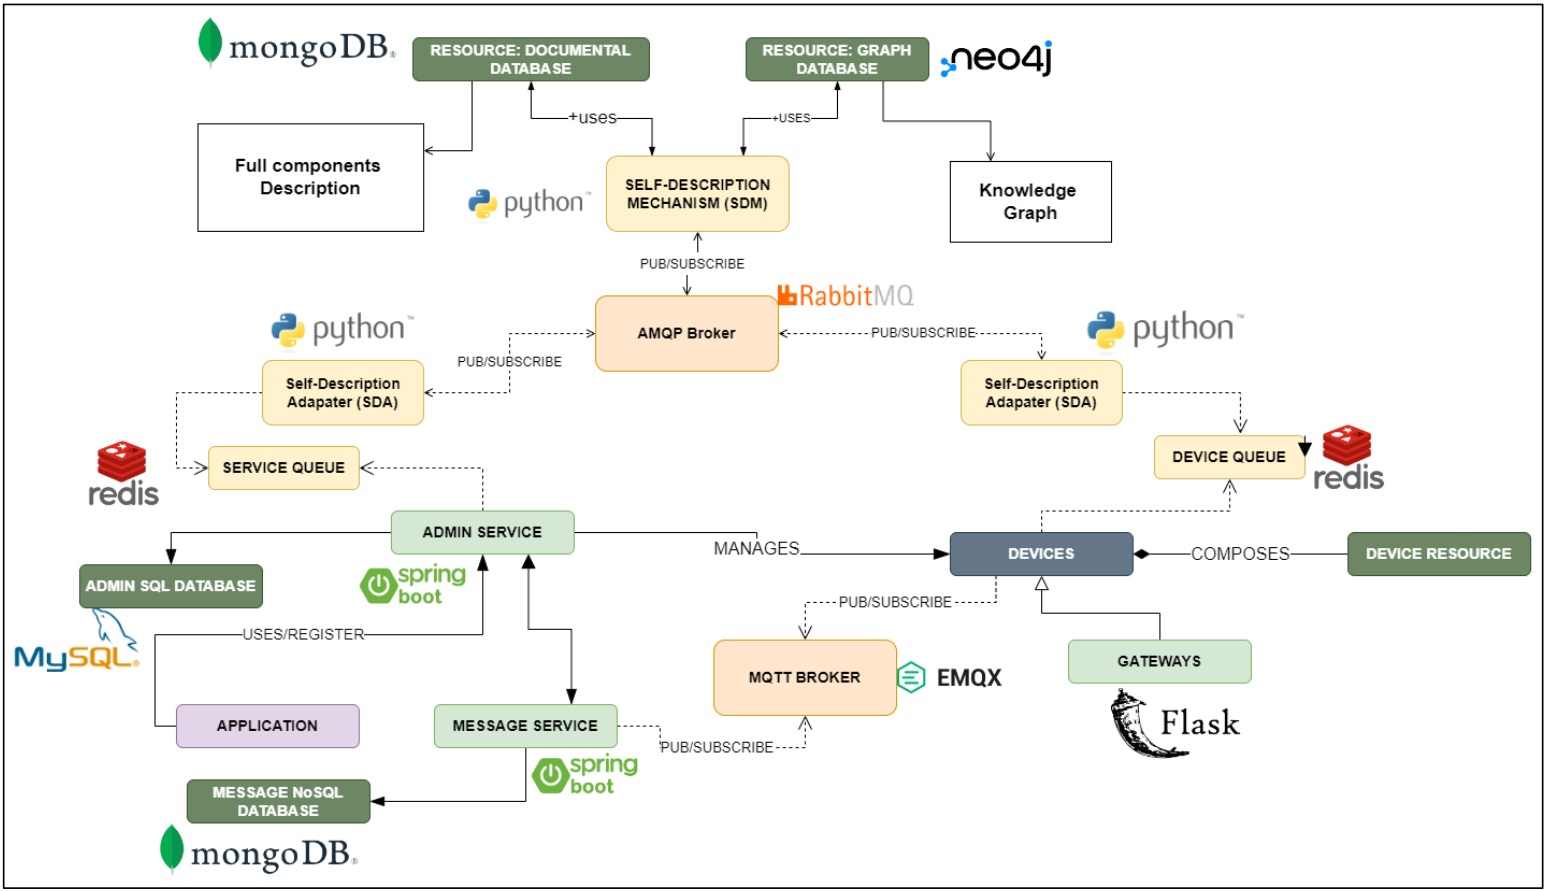
\includegraphics[width=\linewidth]{images/ArquitecturaSmartCampus.png}
    \label{fig:ArquitecturaSmartCampus}
\end{figure}


Ahora, cada una de las maneras de acceder a los datos es viable, y podría permitir la implementación correspondiente para determinar el estado del sistema. Sin embargo, de entre las tres opciones, se escogió el procesamiento de los mensajes enviados por los dispositivos, enviados por MQTT. Esta decisión se debe a algunas de las ventajas que posee el protocolo sobre la consulta a base de datos. Entre estas destacan la menor latencia en la recuperación y la direccionalidad de datos, comparado con las consultas. 

La primera se refiere a la menor cantidad de saltos de servicios antes de que los datos sean guardados en la base de datos, lo que aumenta el tiempo en el que estos estarán disponibles, sumado a el tiempo ejecución de la consulta. Así mismo, la última refiriéndose a que el protocolo MQTT, gracias a su modelo pub/sub, permite el poder procesar los datos a medida que estos van llegando, y no en intervalos discretos de tiempo, lo cual podría afectar la toma de decisiones.

Partiendo de lo anterior, se reconoció la necesidad de tener un servicio dedicado a la tarea de procesar los mensajes que están siendo enviados por, y a, cada uno de los dispositivos registrados en Smart Campus UIS. 

\subsection{Implementado un Event-Handler}

En el contexto de Smart Campus UIS, podemos ver cada uno de los mensajes que se envían los adaptadores de auto-descripción como un evento. Es decir, cada uno de los mensajes que es enviado por los dispositivos pertenecientes a una aplicación de Smart Campus UIS, es algo que debe ser procesado con un algún fin. Este procesamiento, recuerda al patrón de diseño \texttt{Observer} en el cual se busca el realizar una acción cada vez que el estado, de lo que se está observando, cambia.

Siendo así, se estableció el realizar la implementación de un observador el cual se hará responsable de la captura de los mensajes enviados por los dispositivos y establecer el estado del sistema. De esto, como se puede ver en la figura \ref{fig:proceso_looker} se propuso un proceso que debía realizar el observador a implementar.

\begin{figure}[H]
    \caption{Primera propuesta del proceso a realizar \linebreak por el observador a implementar} 
    \centering
    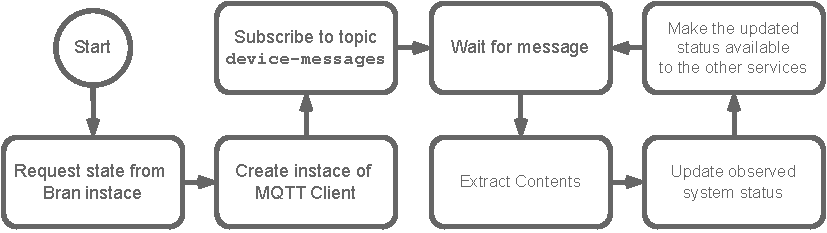
\includegraphics[width=0.6\linewidth]{images/LookerProcess.pdf}
    \label{fig:proceso_looker}
\end{figure}

Este primer acercamiento, es bastante directo en cuanto a la implementación a realizar. Esta se basa en la inicialización de un cliente de MQTT, subscrito al tópico usado por los dispositivos conectados a Smart Campus \cite{SmartCampusGithub}, y procesar cada uno de los mensajes a medida que estos van llegando.

% Ask mom, I really don't know if problem next to solution or problems them solution

% New section here?

En este primer prototipo de nuestro observador, existen algunas limitaciones a resolver. El primero de estas que no le da acceso al observador, de aquí en adelante referido como \textit{Looker}, acceder al contexto geográfico, requerido para evaluar el estado de cada una de las locaciones de la aplicación. 

Esto se solucionó realizando una petición de la descripción del campus, requerido para la declaración del estado objetivo, a un endpoint que tenga estos datos. Para su implementación fue necesario realizar una modificación a Lexical para que este, tras validar la arquitectura objetivo, envíe el resultado serializado a un servicio encargado de almacenar las arquitecturas objetivo. 

De la misma manera, quedaba pendiente el definir el como los demás servicios podrán acceder a los datos que están siendo procesados. Es decir, si vamos a usar un bus de datos para publicar el estado del sistema al resto de nuestros servicios, o permitir el acceso con peticiones HTTP a través de un endpoint.

La implementación de esto depende del como se desee realizar el manejo de los cambios en la arquitectura de Smart Campus UIS. Si se desea responder de manera inmediata a cambios en la arquitectura, se tendría que usar un bus de datos, como MQTT o AMQP; pero tendría la consecuencia de un aumento en el uso de los recursos debido a que se tendrían que procesar todos los cambios cada vez que se determine el estado de la aplicación. 

En el caso contrario, podría implementarse un endpoint HTTP el cual sea consultado en intervalos de tiempo por el servicio encargado de comparar los estados objetivo y de referencia. Esto permitiría tener un mayor control de cada cuanto se realizan las comparaciones, y más importante, cada cuanto se realizan acciones sobre la arquitectura actual con el fin de modificarla hacia el estado de referencia.

Siendo así, y debido a querer manejar más el control desde el servicio encargado de los cambios en la arquitectura, que se escogió la opción de emplear un endpoint. De esta manera, se podrá regular cada cuanto se realizan acciones sobre Smart Campus UIS, lo que debería resultar en un comportamiento más predecible.

Finalmente, este primer prototipo, no establece el como se realizará la evaluación del estado del sistema. De no tener una métrica la cual evaluar, no se habrá manera de detectar las diferentes alteraciones al estado actual del sistema.

Para esto, del contexto proveído, se tomaron las propiedades con el fin de establecer el estado de un componente. Ahora, a pesar de considerar otros parámetros y puntos de medida para nuestro servicio, debido a la gran cantidad de necesidades que pudiera presentar un usuario final, como lo pueden ser el mantener datos en un rango o la distribución entre estos; se decidió, para efectos de esta implementación inicial, sólo tomar como parámetros básicos el tiempo entre mensajes de los dispositivos y la cantidad de estos en una locación. La nueva estructura del proyecto, hasta el momento, puede observarse en la figura \ref{fig:StarDuckBasic}.
 
% Esta primera parte se solucionó realizando una petición de la descripción del campus, requerido para la declaración del estado objetivo, a un endpoint que tenga estos datos. Para su implementación fue necesario realizar una modificación a Lexical para que este, tras validar la arquitectura objetivo, envíe el resultado serializado a un servicio encargado de almacenar las arquitecturas objetivo. La nueva estructura del proyecto, hasta el momento, puede observarse en la figura \ref{fig:StarDuckBasic}.

\begin{figure}[ht]
    \centering
    \caption{Arquitectura actual del proyecto}
    \label{fig:StarDuckBasic}
    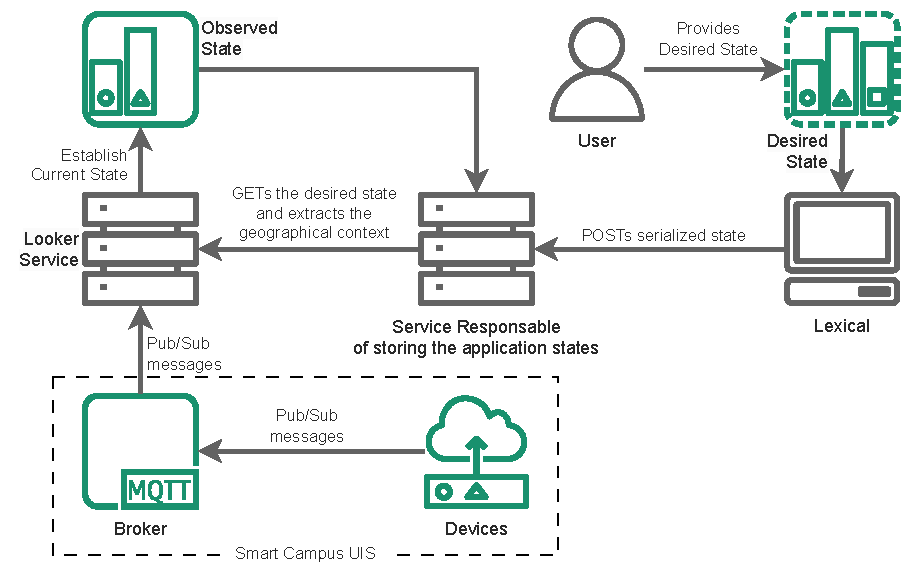
\includegraphics[width=\linewidth]{images/StarDuckBasic.pdf}
\end{figure}

% Respecto al segundo punto, la implementación de este depende del como se desee realizar el manejo de los cambios en la arquitectura de Smart Campus UIS. Si se desea responder de manera inmediata a cambios en la arquitectura, se tendría que usar un bus de datos, como MQTT o AMQP; pero tendría la consecuencia de un aumento en el uso de los recursos debido a que se tendrían que procesar todos los cambios cada vez que se determine el estado de la aplicación. 

% En el caso contrario, podría implementarse un endpoint HTTP el cual sea consultado en intervalos de tiempo por el servicio encargado de comparar los estados objetivo y de referencia. Esto permitiría tener un mayor control de cada cuanto se realizan las comparaciones, y más importante, cada cuanto se realizan acciones sobre la arquitectura actual con el fin de modificarla hacia el estado de referencia.

% Siendo así, y debido a querer manejar más el control desde el servicio encargado de los cambios en la arquitectura, que se escogió la opción de emplear un endpoint. De esta manera, se podrá regular cada cuanto se realizan acciones sobre Smart Campus UIS, lo que debería resultar en un comportamiento más predecible.

% Ahora, en cuanto a la manera en la que se evaluará el estado de los diferentes orígenes de datos. Para esto, del contexto proveído, se tomaron las propiedades con el fin de establecer el estado de un componente. Ahora, a pesar de considerar otros parámetros y puntos de medida para nuestro servicio, debido a la gran cantidad de necesidades que pudiera presentar un usuario final, como lo pueden ser el mantener datos en un rango o la distribución entre estos; se decidió, para efectos de esta implementación inicial, sólo tomar como parámetros básicos el tiempo entre mensajes de los dispositivos y la cantidad de estos en una locación. 

\subsection{Comparando Arquitecturas}

Ahora que se conoce el estado actual del sistema, al igual que estado de referencia; lo siguiente a realizar era la comparación de las arquitecturas. El resultado de esta, nos daría la base para poder decidir el qué hacer para adaptar el sistema y el cómo hacerlo.

En la figura \ref{fig:StarDuckBasic}, uno de los servicios intermedios estaba encargado de manejar la base de conocimiento. Este contiene las versiones actualizadas de la arquitectura de referencia, enviada a este desde el cliente de Lexical usado por el usuario; y el estado actual, que Looker está constantemente actualizando, y puede ser consultado por este servicio cada que se requiera. Siendo así, este servicio será el encargado de realizar las comparaciones entre los dos estados.

Ya teniendo definido dónde se realizarán las comparaciones, lo siguiente es definir el como se realizarán estas. Para nuestras necesidades, esto no es tan directo como hacer una comparación usando un igual (\texttt{A == B}) ya que el realizar esto, no nos daría realmente información sobre, qué, internamente, presenta problemas.

Para poder extraer esta información, siendo esta el estado de los componentes específicos que necesitan atendidos, se estableció el uso de métricas definidas con anterioridad. En este caso, las métricas elegidas son el tiempo entre mensajes de los dispositivos y la cantidad de estos en una locación.

El proceso de comparación consta de evaluar cada componente del sistema en función de estas métricas. Se comparan las versiones objetivo y actual para determinar si hay discrepancias significativas que requieran ajustes. Si, por ejemplo, el tiempo entre mensajes de un dispositivo en una ubicación difiere de la versión objetivo, se considera que hay una desviación. Lo mismo ocurre si la cantidad de dispositivos en una locación no coincide con la definición de la arquitectura objetivo.

Lo siguiente a realizar fue definir el proceso de comparación entre los dos estados del sistema. Se optó por abordar esta comparación locación por locación, permitiendo así una evaluación detallada de cada área y extrayendo una estructura que resaltara los puntos problemáticos de la aplicación y las diferencias presentes en cada uno de los lugares. 

Siendo así, primeramente se definió el flujo en el cual se realizará el recorrido de las locaciones. Se parte desde las locaciones raíces, o de primer nivel, y pasando por cada una de las locaciones hijas revisando el estado de cada una de estas. En la figura \ref{BranProcess} se presenta el diagrama de flujo de la forma en la que se realizará el recorrido de las locaciones.

\begin{figure}[hb]
    \centering
    \caption{Diagrama de flujo del recorrido de las locaciones}
    \label{BranProcess}
    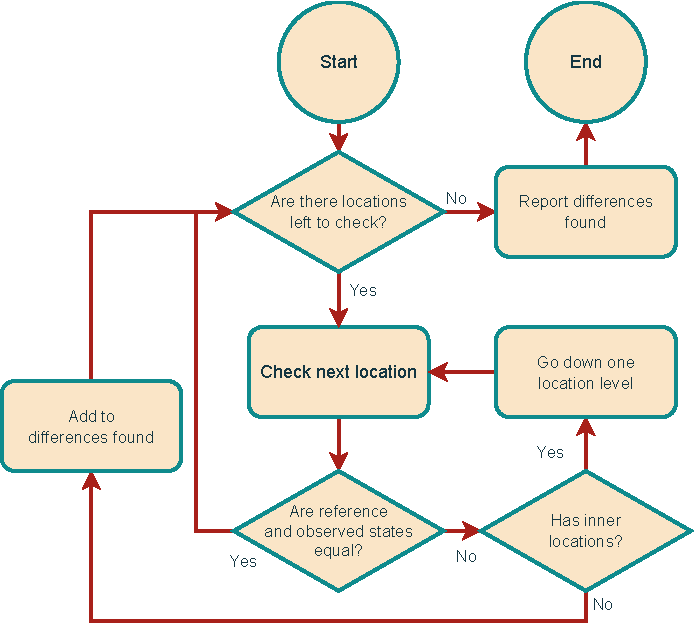
\includegraphics[width=0.9\linewidth]{images/BranProcess.pdf}
\end{figure}

En cada una de las locaciones que se visita, se compara el estado de cada uno de los componentes definidos en la arquitectura de referencia. Esta comparación se basa en revisar tres cosas. Primero, si el componente está presente en la locación; segundo, como fue definido en la sección anterior, si se han estado mandando mensajes dentro del tiempo establecido; y, finalmente, si se está recibiendo el tipo de dato esperado.

Estos puntos de comparación nos permiten establecer si el componente está presente y activo en la locación; al igual que el tipo de| dato registrados sean coherentes con las necesidades de la aplicación. El diagrama de flujo del proceso defino se puede observar en la figura \ref{fig:BranCompare}.

\begin{figure}[ht]
    \centering
    \caption{Diagrama de flujo del proceso de comparación de los componentes}
    \label{fig:BranCompare}
\end{figure}